\documentclass[10pt,twocolumn,letterpaper]{article}

\usepackage{cvpr}
\usepackage{times}
\usepackage{epsfig}
\usepackage{graphicx}
\usepackage{amsmath}
\usepackage{amssymb}

% Include other packages here, before hyperref.

% If you comment hyperref and then uncomment it, you should delete
% egpaper.aux before re-running latex.  (Or just hit 'q' on the first latex
% run, let it finish, and you should be clear).
\usepackage[pagebackref=true,breaklinks=true,letterpaper=true,colorlinks,bookmarks=false]{hyperref}

%\cvprfinalcopy % *** Uncomment this line for the final submission

\def\cvprPaperID{****} % *** Enter the CVPR Paper ID here
\def\httilde{\mbox{\tt\raisebox{-.5ex}{\symbol{126}}}}

% Pages are numbered in submission mode, and unnumbered in camera-ready
\ifcvprfinal\pagestyle{empty}\fi
\begin{document}

%%%%%%%%% TITLE
\title{Task 3 \& Task 4: Classifying gender & Age Image Regression }

\author{Konstantinos Katergaris\\
Arizona State University\\
1151 S Forest Ave, Tempe, AZ\\
{\tt\small kkaterga@asu.edu}}

%\thispagestyle{empty}

\maketitle

\section{Task 3}

\subsection{Introduction}
In this section, the task was to classify the gender of a patient based on an X-ray image. The task was initially approached by replacing the classification head with the appropriate number of classes on a pretrained model, specifically a SWIN-Transformer V2 with a window size of 7 and an input size of 256x256, by Microsoft. As this is a simple binary classification problem, random augmentations were introduced to potentially improve the model's performance, given the small dataset size. The idea was that augmentations would artificially increase the number of data points and enhance generalization. However, contrary to this hypothesis, the data augmentations led to worse results.
\subsection{Dataset}
The dataset used \cite{DatasetForClass} consists of chest X-ray images in JPG format with RGB color channels and a resolution of 256x256 pixels. It includes 2 classes: female and male. The dataset contains a total of 247 images, but the classes are imbalanced. In the test set, consisting of 93 samples, 42 were female and 51 were male. In the training set, which contains 154 samples, 86 were female and 68 were male. The dataset was loaded into the model using the Huggingface library's dataset object \cite{huggingfacedataset}. Additionally, it was noted that some of the test data may be incorrectly labeled.

\subsection{Training}
The model was trained using the Huggingface Transformers Trainer \cite{huggingfacetrain}. The optimal hyperparameters, determined during training without augmentations, were a learning rate of 5e-4, a batch size of 4, and 50 epochs. This configuration resulted in an accuracy of 0.9247 and an AUC of 0.9272.
\subsection{Image Preprocessing}
The images from the dataset were processed using the AutoImageProcess function from the Huggingface Transformers library \cite{huggingfaceproc}, applying its default pretrained configurations \cite{huggingface}. This function automated various preprocessing steps, including resizing, as well as other procedures defined in the original model’s configuration.

\subsection{Experiments}
To test if data augmentations would help the results of the model pytorches transforms library was used\cite{}. The following augmentation where applied to the dataset at random: horizonatal flip, vertical flip, and rotation of $30^{\circ}$. Furthermore, the AutoImageProcess function \cite{huggingfaceproc} to first apply the new augmentations before completing the regular preproccesing steps.


\subsection{Results}
The following Table ~\ref{tab:augmentations_results} shows the test accuracy and AUC of the model with and without augmentations and the following figures are confusion matrices of their predictions Figure ~\ref{fig:og_confusion} and Figure ~\ref{fig:augmented}.

\begin{table}[h!]
\centering
\begin{tabular}{l|c|c|}
\hline
\bf{Run} & \bf{Accuracy} & \bf{AUC}  \\ \hline
Without Augmentations & 0.9247 & 0.9272 \\ \hline
With Augmentations & 0.8495 & 0.8438 \\ \hline
\label{tab:ACC}
\end{tabular}

\caption{Comparison of Accuracy and AUC with and without Data Augmentations}
\label{tab:augmentations_results}
\end{table}

\begin{figure}[h!]
    \centering
    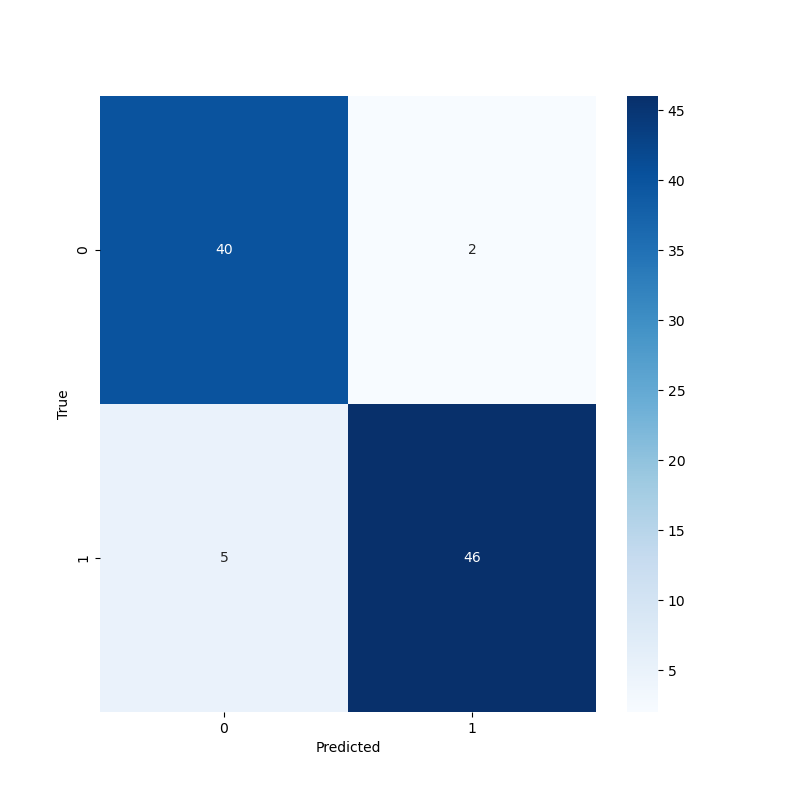
\includegraphics[width=1\linewidth]{image.png}
    \caption{Confusion matrix of the model without augmentations. 0 representing female, and 1 representing male }
    \label{fig:og_confusion}
\end{figure}
\begin{figure}[h!]
    \centering
    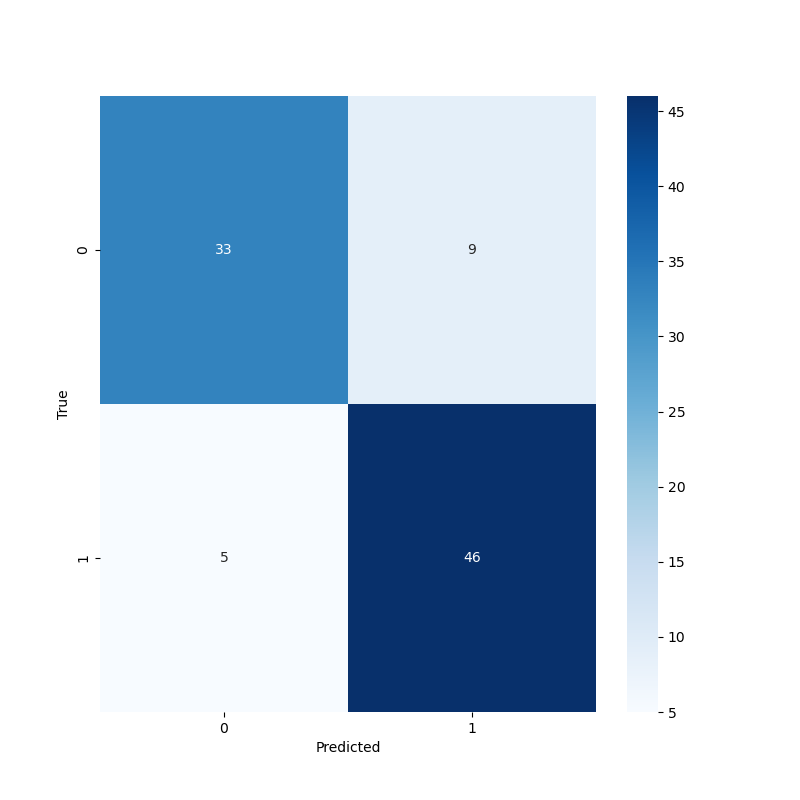
\includegraphics[width=1\linewidth]{image_1.png}
    \caption{Confusion matrix of the model with augmentations. 0 representing female, and 1 representing male}
    \label{fig:augmented}
\end{figure}
\subsection{Conclusion}
Contrary to the hypothesis, the augmentations didn't improve performance in the models. Instead, they made them worse by about 10\% accuracy. This is probably due to the miss labeled samples in the test set.
\newpage
\subsection{Introduction}
The task involved developing a model to determine a patient's age based on chest X-ray images. Initially, a pretrained Tiny SWIN-Transformer V2, with a window size of 7 and an input size of 256x256, developed by Microsoft, was used. Its classification head was replaced with a linear layer, as the task was framed as an image regression problem. In image regression, the model is trained to predict a continuous value rather than a discrete label. To explore alternative approaches, a modified ResNet34 model, originally designed for age regression on facial images, was also researched and implemented \cite{medium_age_prediction}.


\subsection{Dataset}
The dataset used \cite{DatasetForClass} consists of chest X-ray images in JPG format with RGB color channels and a resolution of 2048x2048 pixels. It contains a total of 247 images, with 81 used for training and 168 for testing. Each split contains a random selection of patients aged between 16 and 90. The dataset splits were provided via two CSV files—one for the training set and one for the test set—each containing two columns: one for the image paths and the other for the patients' ages. A custom dataset class was created by subclassing PyTorch's Dataset object. This allowed the image paths and ages to be passed to the model by deconstructing a pandas DataFrame, which was used to load the CSV files. Furthermore, age values were normalized for smooth training.
\subsection{Model}
The model used was provided by \cite{medium_age_prediction}, which is a ResNet34 model modified by the author to remove its classification-specific layers. While the author did not provide detailed information on the exact modifications, further details on the model can be found in \cite{medium_age_prediction}. An important aspect of the model is the adjustment of the final layer, where the output was "squeezed" along the last dimension. This removes dimensionality from the output tensor, effectively flattening the model’s output to a value from 0-1.

\subsection{Training}
\subsubsection{Image Preprocessing}
Each image was resized to 244x244 pixels, which is the expected input size for the ResNet34 model. Additionally, the images were normalized.

\subsubsection{Hyperparameters}
The authors used Fastai, a Python library that simplifies the process of model training, to train the model. However, a custom training loop was implemented for greater control over the training process. The Adam optimizer was used with a learning rate of 5e-5 and a weight decay of 0.01 to help mitigate the high variance in the data. Additionally, a OneCycleLR scheduler was employed to dynamically adjust the learning rate during training, which aids in better convergence and helps avoid local minima. The model was trained for 50 epochs, with gradient clipping applied to a maximum norm of 2.0 to prevent exploding gradients and ensure smoother training. The L1LossFlat loss function was used per the paper.

\subsection{Results}
The following table where my results measured in MAE and RMSE since it is a regression problem :
\begin{table}[h!]
\centering
\begin{tabular}{|c|c|}
\hline
 \bf{MAE} & \bf{RMSE} \\ \hline
 7.9477 & 10.1413 \\ \hline
\end{tabular}
\caption{ MAE and RMSE Results }
\label{tab:best_results}
\end{table}





{\small
\bibliographystyle{ieee_fullname}
\bibliography{egbib}

}
\end{document}
